\documentclass[a4paper, 10pt, oneside]{article}
\renewcommand{\familydefault}{\sfdefault}
%---------------------------------------------------------------------------------
%------------------------- Set the variables for the Mainpage here ---------------
%---------------------------------------------------------------------------------
\newcommand{\name}{Your Name}
\newcommand{\email}{your.email@domain.tld}
\newcommand{\osid}{OS-XXXXX}

%---------------------------------------------------------------------------------
%------------------------- Include the list of used packages ---------------------
%---------------------------------------------------------------------------------
\usepackage{lastpage}
\usepackage{tabularx}
\usepackage{cprotect}
%Seitenränder definieren
\usepackage[right=2.8cm,left=2.5cm, bottom=3.9cm, top=4.1cm, footskip=2.1cm, headsep=2.0cm]{geometry}
\usepackage[utf8]{inputenc}
\usepackage[T1]{fontenc}
\usepackage{palatino}
\linespread{1.25}
\usepackage{microtype}
\usepackage[english]{babel}
%More citations
\usepackage{natbib}
%better urls mit \url{}
\usepackage[hyphens]{url}
\usepackage{lastpage}
%code
\usepackage{listings}

%more colors
\usepackage{soul}

%Force figure to be placed “HERE”
\usepackage{float} 

%folgende Zeilen sind für Kapitelüberschriften
\usepackage[rigidchapters]{titlesec}
\usepackage{blindtext}
\titleformat{\chapter}
{\normalfont\LARGE}
{\makebox[3pc][l]{\LARGE\thechapter\hfil\rule[-6pt]{0.5pt}{2pc}}}
{0pt}
{\LARGE}
\titlespacing*{\chapter}{0pt}{0pt}{82pt}

%Csv -> Latex
\usepackage{csvsimple}



%Für Graphiken 
\usepackage{tikz}
\usetikzlibrary{plotmarks}
\usetikzlibrary{positioning,shapes,shadows,arrows}
\usepackage{graphicx}

%Paket gibt einige Optionen mehr bei Tabellen (wird eher nicht verwendet)
\usepackage{array}

%\usepackage{stdpage}
%test wegen anzahl zeilen pro seite
%Paket für Zeilenabstände
\usepackage{setspace}
%\onehalfspacing
\usepackage{multirow}
%Paket gibt mehr Kontrolle über die Captions (Bildunterschriften) bei Abbildungen
\usepackage[labelfont=bf,format=hang,font=footnotesize,justification=centering,singlelinecheck=false]{caption}
\usepackage{subcaption}

%Helvetia (Arial) Verwenden WICHTIG: Beide folgenden Zeilen kopieren!
%\usepackage[scaled]{helvet} %
%\renewcommand*\familydefault{\sfdefault} %%

% Abschalten des Einrückens bei neuen Absätzen (manuell, nach Tabellen, Abbildungen, etc.)
\setlength{\parindent}{0pt}
\hyphenation{}

% New Page before section
\newcommand{\sectionbreak}{\clearpage}

\usepackage{color}

\definecolor{color0}{rgb}{0,0,0}% black
\definecolor{color1}{rgb}{0.22,0.45,0.70}% light blue
\definecolor{color2}{rgb}{0.45,0.45,0.45}% dark grey
\definecolor{mygreen}{rgb}{0,0.6,0}
\definecolor{mygray}{rgb}{0.5,0.5,0.5}
\definecolor{myblue}{rgb}{0.0, 0.53, 0.74}
\definecolor{codebackground}{rgb}{0.8, 0.8, 0.8}
\definecolor{codechanged}{rgb}{0.8, 0.0, 0.0}

\lstset{ %
  backgroundcolor=\color{codebackground},   % choose the background color; you must add \usepackage{color} or \usepackage{xcolor}
  basicstyle=\footnotesize,        % the size of the fonts that are used for the code
  breakatwhitespace=false,         % sets if automatic breaks should only happen at whitespace
  breaklines=true,                 % sets automatic line breaking
  captionpos=b,                    % sets the caption-position to bottom
  commentstyle=\color{mygreen},    % comment style
  deletekeywords={...},            % if you want to delete keywords from the given language
  escapeinside={\%*}{*)},          % if you want to add LaTeX within your code
  extendedchars=true,              % lets you use non-ASCII characters; for 8-bits encodings only, does not work with UTF-8
% frame=single,	                   % adds a frame around the code
  keepspaces=true,                 % keeps spaces in text, useful for keeping indentation of code (possibly needs columns=flexible)
  captionpos=bc,
  breaklines=true,
% keywordstyle=\color{blue},       % keyword style
% language=Octave,                 % the language of the code
% otherkeywords={*,...},           % if you want to add more keywords to the set
  numbers=left,                    % where to put the line-numbers; possible values are (none, left, right)
  numbersep=5pt,                   % how far the line-numbers are from the code
  numberstyle=\tiny\color{mygray}, % the style that is used for the line-numbers
  rulecolor=\color{black},         % if not set, the frame-color may be changed on line-breaks within not-black text (e.g. comments (green here))
  showspaces=false,                % show spaces everywhere adding particular underscores; it overrides 'showstringspaces'
  showstringspaces=false,          % underline spaces within strings only
  showtabs=false,                  % show tabs within strings adding particular underscores
  stepnumber=2,                    % the step between two line-numbers. If it's 1, each line will be numbered
% stringstyle=\color{mymauve},     % string literal style
  tabsize=2,	                   % sets default tabsize to 2 spaces
% title=\lstname,                   % show the filename of files included with \lstinputlisting; also try caption instead of title
  moredelim=**[is][\color{codechanged}]{**@}{@**}, %Rot für Änderungen
  moredelim=**[is][\color{myblue}]{***@}{@***}, %einfaches blau
  moredelim=**[is][\color{mygreen}]{*@}{@*},%einfaches Grün
}

%Aktives Inhaltsverzeichnis und links
\usepackage{hyperref}
\hypersetup{
    colorlinks,
    citecolor=black,
    filecolor=black,
    linkcolor=black,
    urlcolor=black
}

\usepackage{fancyhdr}
\pagestyle{fancy}
\fancypagestyle{plain}{}
\fancyhf{}
\fancyfoot{} % clear all footer fields

\fancyhead[R]{\small{\leftmark}}
\fancyhead[L]{\small{Offensive Security - Penetration Test Report}}
\renewcommand{\sectionmark}[1]{\markboth{#1}{}}

\renewcommand{\footrulewidth}{0.1pt} % Create a rule above the page number
\fancyfoot[R]{\textcolor{color1}\thepage  \textcolor{color2}{/\pageref{LastPage}}}

\makeatletter
\g@addto@macro\@floatboxreset\centering
\setlength{\@fptop}{5pt}
\makeatother
\catcode`\_=12
\usepackage{fancyvrb}
\newcommand{\footnoteref}[1]{\footnote{See footnote \ref{#1}.}}
\newcommand{\fullhostname}{\textit{\hostname\ (\ip)}}
\usepackage{tabularx}
\newcommand{\simpleref}[1]{\hyperref[#1]{#1}}
\newcommand{\definevuln}[2]{\DeclareRobustCommand{#1}{\textit{#2}}}
\newcommand{\definevulnf}[3]{\DeclareRobustCommand{#1}{\textit{#2}\footnote{#3}}}

\setlength{\parskip}{1em}

%\usepackage[htt]{hyphenat} 

%---------------------------------------------------------------------------------
%------------------------- Create title page -------------------------------------
%---------------------------------------------------------------------------------
\title{{\textbf{\Huge Offensive Security}}\\Penetration Test Report for\\OSCP Exam}
\author{\vspace{.8cm}\\{\LARGE \name}\\[1em]\email\\[1em]OSID: \osid}
\date{\vspace{1cm}
\includegraphics{offsec_logo.png}\\\vspace{2cm} \today\\ \vspace{.25cm} \textcopyright\\\vspace{.25cm}
{\small All rights reserved to Offensive Security, 2020\\
No part of this publication, in whole or in part, may be reproduced, copied, transferred or any other right reserved to its copyright owner, including photocopying and all other copying, any transfer or transmission using any network or other means of communication, any broadcast for distant learning, in any form or by any means such as any information storage, transmission or retrieval system, without prior written permission from Offensive Security.}
}

\newcounter{exercisecounter}

\begin{document}
%---------------------------------------------------------------------------------
%------------------------- Print title page --------------------------------------
%---------------------------------------------------------------------------------
\maketitle
\thispagestyle{empty}
%---------------------------------------------------------------------------------
%------------------------- Print table of contents -------------------------------
%---------------------------------------------------------------------------------
% Attention: Document might need some runs to get all indexes etc right .. usual LaTeX stuff :)
\tableofcontents
\thispagestyle{empty}
\pagebreak 

%---------------------------------------------------------------------------------
%------------------------- Exercice counter --------------------------------------
%---------------------------------------------------------------------------------
\setcounter{exercisecounter}{0}
\newcommand{\exercisesection}{\stepcounter{exercisecounter}\subsubsection*{Chapter \theexercisecounter}}

%---------------------------------------------------------------------------------
%------------------------- Declaring the empty variables for the hosts -----------
%---------------------------------------------------------------------------------
\newcommand{\hostname}{}
\newcommand{\ip}{}
\newcommand{\tcpports}{} 
\newcommand{\udpports}{} 
\newcommand{\os}{}
\newcommand{\vuln}{}
\newcommand{\product}{}
\newcommand{\vulnx}{}
\newcommand{\productx}{}
\newcommand{\client}{\textit{kali (ZZ.ZZ.ZZ.ZZ)}}

\section{Executive Summary}
\osid\ was tasked with performing an internal penetration test of the OSCP exam network. An internal penetration test is a simulated attack against internally connected systems. The focus of this test is to perform attacks, similar to those of a malicious entity, and attempt to infiltrate Offensive Security’s internal exam systems.

\osid's overall objective was to find and exploit vulnerabilities while reporting the findings back to Offensive Security. While conducting the internal penetration test, there were several alarming vulnerabilities that were identified within the exam network. 

\par \osid\ was able to gain administrative access to several machines due to vulnerable applications and poor security configurations. The potential for this access can be mitigated by doing stuff.

\section{Overview}
\section{Introduction}
This penetration test report contains all the steps taken to successfully compromise machines in the Offensive Security Certified Professional (OSCP) exam environment; data such as proof of concepts (PoC), custom exploit code, and step-by-step documentation are included. The purpose of this report is to convey the student's understanding of penetration testing methodologies as well as the technical knowledge required to successfully achieve the Offensive Security Certified Professional (OSCP) certification.

\textit{Note: This document serves as a template for the real report; it provides organized presentation so you can focus on pwning boxes. Please read the \href{https://support.offensive-security.com/oscp-exam-guide/}{OSCP Exam Guide} for the composition of your report. Good luck and try harder!}

\section{Results}
\subsection{Scope}
The scope of the penetration test was the OSCP exam network. Below is the list of hosts targeted by \osid.
\begin{itemize}
	\item XX.XX.XX.XX
\end{itemize}


\subsection{Summary of Findings}

Using the \client{} machine, \osid{} gained administrative access to several machines by exploiting their vulnerabilities. These machines and their vulnerabilities are listed below and further documented in section~\ref{sec:hosts}. Table~\ref{tab:summary_vuln} summarizes the findings.

%Define vulnerabilities below for referencing throughout the report
%-----------------Vulnerabilities-------------------%
\definevuln{\vulnPassword}{Weak User Password}
% \definevulnf also adds a footnote with the 2nd parameter
\definevulnf{\vulnCow}{Dirty Cow Privilege Escalation}{\url{https://dirtycow.ninja/}}
%----------------------------------------------------%

% Technical rundown of hosts and their vulnerabilities
%\begin{center}


\begin{table}[th]
\begin{tabularx}{\textwidth}{|l|l|X|}
    \hline
    Hostname & IP & Vulnerability \\ 
    \hline
    \simpleref{example} & XX.XX.XX.XX & 
    \vulnPassword \newline 
    \vulnCow \\
    \hline
\end{tabularx}
\label{tab:summary_vuln}
\caption{Dirty Cow.}
\end{table}

%\end{center} 
\subsection{Detailed findings}
This section details the relevant findings for each host that were in the scope of this assessment.
%----------BOX_RUNDOWNS---------%
% !TeX spellcheck = en_US

%--------------------------Set the variables for every client---------------------
\renewcommand{\hostname}{machineA}
\renewcommand{\os}{\textit{Ubuntu 16.04 LTS}}
\renewcommand{\ip}{XX.XX.XX.XX}

\renewcommand{\vuln}{}
\renewcommand{\product}{}
%The x-Variables are only used, when root is defined (== root shell)
\renewcommand{\vulnx}{\vulnPassword}
\renewcommand{\productx}{}
%%%Did you get root? Comment out if you only got low priv access 
\def\gotroot{}   %%% Define root if you got root shell
%\undef\gotroot % Else undefine

%-------------------------------Auto generated content-----------------------------%----------------------------------------------------------------------------------
\subsection{\label{\hostname}\hostname}

\textit{Note: This machine is fictional and unrelated to Offensive Security machines. Details have been fabricated for purposes of example.}

\subsubsection{Service Enumeration}

\ip\ was scanned with the following switches and relevant output:
\par \texttt{nmap -iL targets -A -oA basicscan}

\begin{lstlisting}[caption={Nmap scan},label={lst:nmap}]
	...
	Nmap scan report for XX.XX.XX.XX
	Host is up (0.12s latency).
	Not shown: 998 closed ports
	PORT   STATE SERVICE VERSION
	...
	80/tcp open  http    Apache httpd 2.4 ((Ubuntu))
	...
\end{lstlisting}



%-------------------------------REMOTE ACCESS---------------------------------

\subsubsection{Remote Access Exploitation}

\paragraph{Vulnerability Discussion} 
% Using \vulnPassword defined in maindocument.tex
\vulnPassword: Malicious users can upload a reverse shell through the backend management interface by exploiting weak administrative credentials.

\paragraph{Recommendations}
Inform users about the importance of strong authentication to security efforts\footnote{Official Microsoft password guidance: \url{https://www.microsoft.com/en-us/research/wp-content/uploads/2016/06/Microsoft_Password_Guidance-1.pdf}}. Additionally, disable remote web access to the management interface.


\paragraph{Proof of Concept}

\osid\ searched for attack vectors in \fullhostname's web services by using Gobuster to brute force files and directories on \url{http://XX.XX.XX.XX}.\\
\texttt{gobuster dir -w /var/lists/dirbuster_medium --url http://XX.XX.XX.XX}
\begin{lstlisting}[caption={Gobuster output.}, label={lst:gobuster}]
	===============================================================
	Gobuster v3.0.1
	by OJ Reeves (@TheColonial) & Christian Mehlmauer (@_FireFart_)
	===============================================================
	[+] Url:            http://XX.XX.XX.XX
	[+] Threads:        20
	[+] Wordlist:       /var/lists/dirbuster_medium
	[+] Status codes:   200,204,301,302,307,401,403
	[+] User Agent:     gobuster/3.0.1
	[+] Extensions:     php
	[+] Timeout:        10s
	===============================================================
	2020/04/20 00:04:20 Starting gobuster
	===============================================================
	/index.php (Status: 200)
	/example_backdoor.php (Status: 200)
	===============================================================
	2020/04/20 00:04:20 Finished
	===============================================================	
\end{lstlisting}

Browsing to \url{http://XX.XX.XX.XX//example_backdoor.php} retrieved a management interface. 
\texttt{} 

\begin{figure}[H]
	\includegraphics [width=.75\textwidth]{./hosts/\hostname/image1.png}
	\caption{Management interface. \\ Note: Image sourced from \nolinkurl{http://www.apachegui.net/images/Control.png}.}
	\label{fig:obviouscreds}
\end{figure}

The management interface authentication used weak credentials. \osid\ logged in with username \texttt{Admin} and password \texttt{Password}.

\osid\ then did stuff to gain a low-privilege remote shell.

After doing stuff, \osid\ exfiltrated evidence of the low-privilege shell.

\begin{figure}[H]
	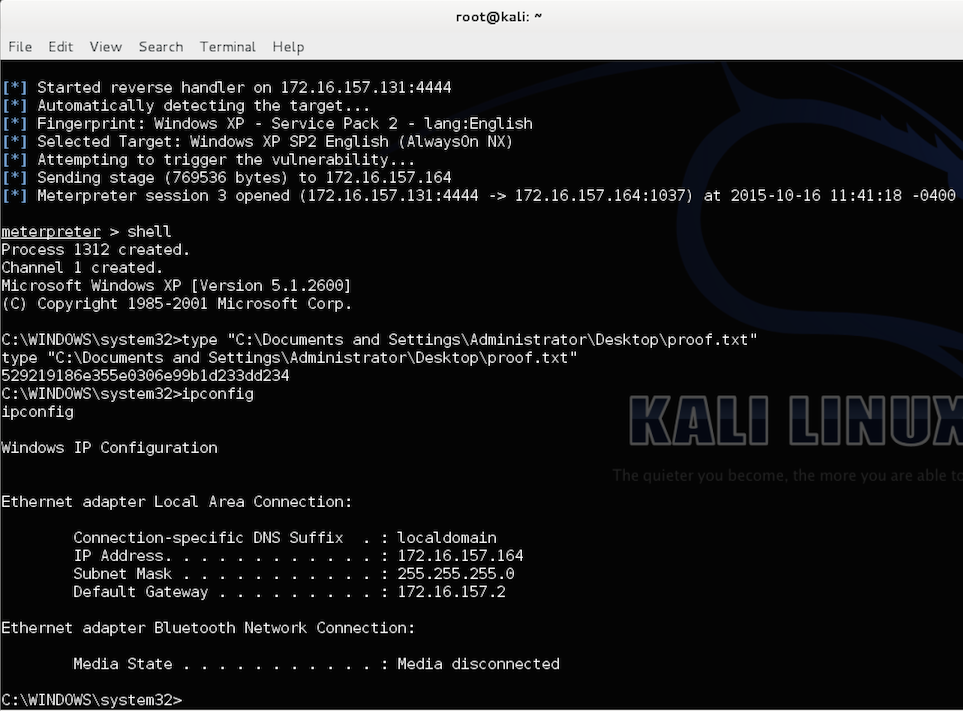
\includegraphics [width=.75\textwidth]{./hosts/\hostname/image2.png}
	\caption{Proof of succesful low-privilege remote access to \fullhostname. \\
		Note: Image sourced from \url{https://support.offensive-security.com/oscp-exam-guide/}. Ensure \texttt{type} or \texttt{cat} are used to print the flag and \texttt{ipconfig} or its counterparts to display the machine's address.}
\end{figure}

%-------------------------------PRIVILEGE ESCALATION---------------------------------
\ifdefined\gotroot
\subsubsection{Privilege Escalation}
\paragraph{Vulnerability Discussion}
\vulnCow\ allows privilege escalation of a low-privilege shell. \osid\ exploited the vulnerability to gain root access on \hostname.
\paragraph{Recommendations}
The vendors of \os\ are aware of the privilege escalation vulnerability\footnote{Official support article: \url{https://ubuntu.com/blog/dirty-cow-was-livepatched-in-ubuntu-within-hours-of-publication}}. Follow vendor instructions to remediate vulnerability.

\paragraph{Proof of Concept}

\osid\ exploited \vulnCow. See \ref{sec:vulnCowDiff} for exploit modification details.

\osid\ was then able to exfiltrate the \nolinkurl{proof.txt} key and network configuration.

\begin{figure}[H]
	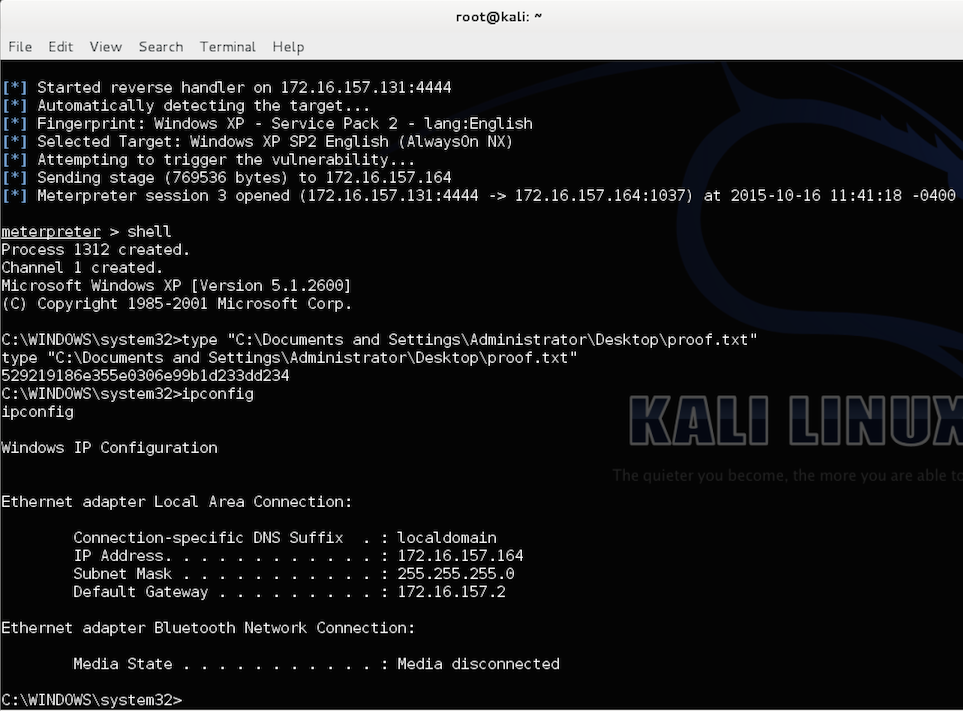
\includegraphics [width=.75\textwidth]{./hosts/\hostname/image2.png}
	\caption{Proof of successful \textit{root} access to \fullhostname. \\Note: Image sourced from \url{https://support.offensive-security.com/oscp-exam-guide/}. Ensure \texttt{type} or \texttt{cat} are used to print the flag and \texttt{ipconfig} or its counterparts to display the machine's address.}
\end{figure}
\fi
%-------------------------------%


\appendix
\section{Appendix}

\subsection{Changes Made to Dirty Cow Exploit}\label{sec:vulnCowDiff}
Additions (green) and subtractions (red) from modification of exploit for \vulnCow. Note: Generated with \url{https://www.diffchecker.com/}.
\begin{figure}[H]
\includegraphics [width=1.0\textwidth]{./appendix/image1.png}
\caption{Dirty cow patch.}
\label{fig:dirtycow}
\end{figure}
\end{document}
